% !TEX encoding = UTF-8
\documentclass{hitgsrep}
\usepackage{graphicx}
\usepackage{amsmath}
\usepackage{physics}
\usepackage[labelformat=simple]{subcaption}
\usepackage{tikz}
%\usepackage[outputdir={out}]{minted}
\usepackage[backend=biber,bibstyle=gb7714-2015,citestyle=gb7714-2015]{biblatex}

\usetikzlibrary{arrows,chains,positioning}

\hitgsrepset{
    author={卢}, % 学生姓名
    studentid={19SXXXXXX}, % 学号
    studentcat={硕士}, % 学生类别
    course={数字信号处理}, % 考核科目
    affiliation={仪器科学与工程学院}, % 学生所在院(系)
    discipline={仪器科学与技术}, % 学生所在学科
    year={2020}, % 年份(不填根据当前时间自动生成,一月时需要手动填入前一年的年份)
    semester={秋}, % 学期(不填根据当前时间自动生成)
}

\ctexset{
    section/format=\Large\bfseries
}

\addbibresource[location=local]{wiener.bib}

\renewcommand\thesubfigure{(\alph{subfigure})} % 得到“图 1(a)”形式的引用
\newcommand{\subjectname}[1]{\begin{center}\LARGE\bfseries #1\end{center}}

\begin{document}
\maketitle

\subjectname{基于维纳滤波对运动模糊图像复原}

\section{运动模糊图像的退化模型}

图像复原问题的关键在于退化模型的建立。
图~\ref{fig:model} 给出了典型的图像退化模型。
如果退化过程是线性空不变的,那么退化过程可以表示为

\begin{equation}\label{eq:model}
    g(x,y)=f(x,y)*h(x,y)+n(x,y)
\end{equation}

\begin{figure}[htb!]
    \centering
    \begin{tikzpicture}[
        font=\small,
        every node/.style={draw, text centered},
        every join/.style={->, draw},
        start chain=going right,
    ]
    \node[on chain] {输入$f(x,y)$}; 
    \node[on chain, join] {$h(x,y)$};
    \node[circle, on chain, join] (sum) {$\sum$};
    \node[on chain, join] {输出$g(x,y)$};
    \node[above=of sum] (noise) {噪声$n(x,y)$};
    \draw[->] (noise) -- (sum);
    \end{tikzpicture}
    \caption{图像退化模型}
    \label{fig:model}
\end{figure}

假设物体 $f(x,y)$ 进行平面运动,$x_0(t)$  和 $y_0(t)$ 分别是在 $x$ 和 $y$ 方向上随时间变化的运动参数,
相机曝光时间为 $\Delta t$,存在加性的高斯白噪声 $n(x,y,t)$。运动模糊得到的像 $g(x,y)$ 满足

\begin{equation}\label{eq:motion}
    \begin{aligned}
        g(x,y)&=\int_0^{\Delta t}\qty{f[x-x_0(t),y-y_0(y)]+n[x-x_0(t),y-y_0(y),t]}\dd{t}\\
        &=\int_0^{\Delta t}f(x,y)*\delta[x-x_0(t),y-y_0(y)]\dd{t}+\int_0^{\Delta t}n[x-x_0(t),y-y_0(y),t]\dd{t}\\
        &=f(x,y)*\int_0^{\Delta t}\delta[x-x_0(t),y-y_0(y)]\dd{t}+\bar{n}(x,y)
    \end{aligned}
\end{equation}
式中的 $\bar{n}(x,y)$ 为噪声 $n(x,y,t)$ 在运动过程中随时间变化得到的平均值。

对比式~\eqref{eq:model} 和式~\eqref{eq:motion} 可以得到运动模糊过程的点扩散函数

\begin{equation}\label{eq:motion-psf-raw}
    h(x,y)=\int_0^{\Delta t}\delta[x-x_0(t),y-y_0(y)]\dd{t}
\end{equation}

若运动为匀速直线运动,那么式~\eqref{eq:motion-psf-raw} 可以写成\cite{_radon_2011}

\begin{equation}\label{eq:motion:psf}
    h(x,y)=\begin{cases}
        \frac{1}{L} & 0\le x\le L\cos\theta, 0\le y\le x\tan\theta\\
        0 & \text{其它}
    \end{cases}
\end{equation}
其中,$\theta$ 指运动方向与水平方向间的夹角,称为运动模糊方向;
$L$ 指运动方向上像素移动的距离,称为运动模糊尺度。

\section{运动模糊图像的复原}

对于有加性噪声的图像退化模型(图~\ref{fig:model}),常使用维纳反卷积滤波的方法对图像进行复原。
维纳滤波器是一种基于最小均方误差准则的最优估计器,其评价函数为

\begin{equation}
    e^2=E[(\hat{f}-f)^2]
\end{equation}
其中,$E[\,\cdot\,]$ 是参数的期望值。

据此得到目标函数在频域的最佳估计为\cite{masters_digital_2009}

\begin{equation}\label{eq:wiener}
    \hat{F}(u,v)=\qty[\frac{1}{H(u,v)}\frac{|H(u,v)|^2}{|H(u,v)|^2+S_n(u,v)/S_f(u,v)}]
\end{equation}
其中,$\hat{F}(u,v)$为图像$f(x,y)$在频域的估计,$H(u,v)$为退化过程的传递函数,$G(u,v)$为退化图像$g(x,y)$的频谱,
$S_n(u,v)$为噪声功率谱,$S_f(u,v)$为未退化图像的功率谱。

从式~\eqref{eq:wiener} 的形式上可以看到,维纳反卷积比起单纯的逆滤波过程$1/H(u,v)$主要增加了为了处理噪声引入的一个修正项。
若退化过程不包含噪声,那么维纳滤波和逆滤波是一致的。
但由于噪声的存在,逆滤波得到的估计为

\begin{equation}
    \hat{F}(u,v)=F(u,v)+\frac{N(u,v)}{H(u,v)}
\end{equation}
其中,$N(u,v)$为噪声频谱。

若退化过程传函$H(u,v)$中包含$0$或接近$0$的部分,那么噪声的作用可能会被极度放大

\section{仿真实验结果与分析}

\begin{figure}[htbp!]
    \centering
    \subcaptionbox{原图像\label{fig:origin}}{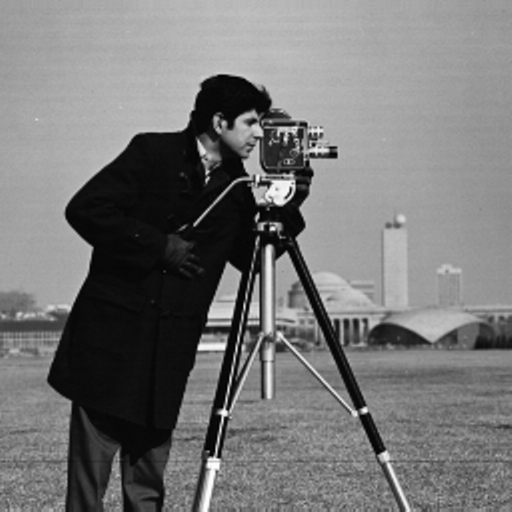
\includegraphics[width=0.32\linewidth]{origin.png}}\hfill
    \subcaptionbox{无噪声的运动模糊图像\label{fig:blurred}}{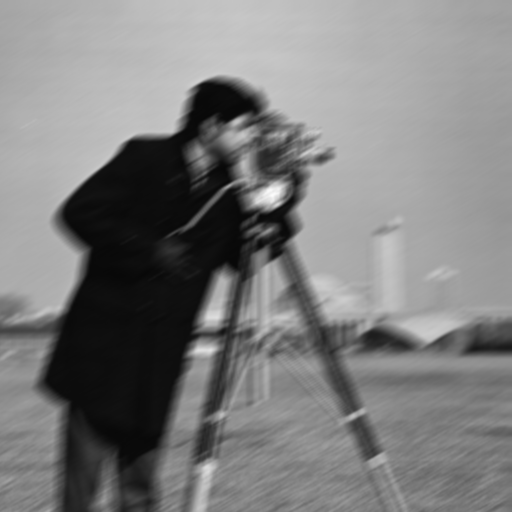
\includegraphics[width=0.32\linewidth]{blurred.png}}\hfill
    \subcaptionbox{图~\ref{fig:blurredn} 逆滤波的结果\label{fig:inverse}}{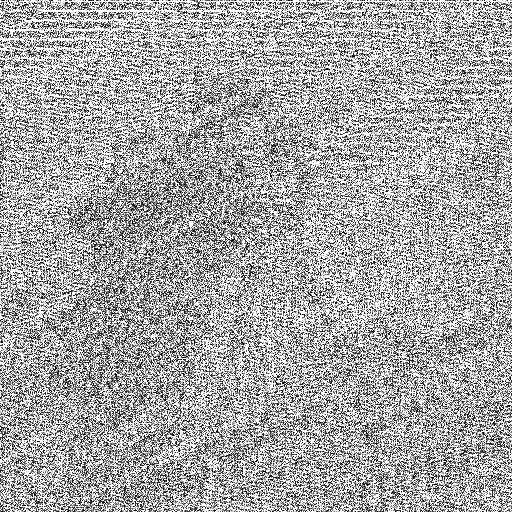
\includegraphics[width=0.32\linewidth]{inverse.png}}\\
    \subcaptionbox{加入$\sigma=0.04$的白噪声的运动模糊图像\label{fig:blurredn}}{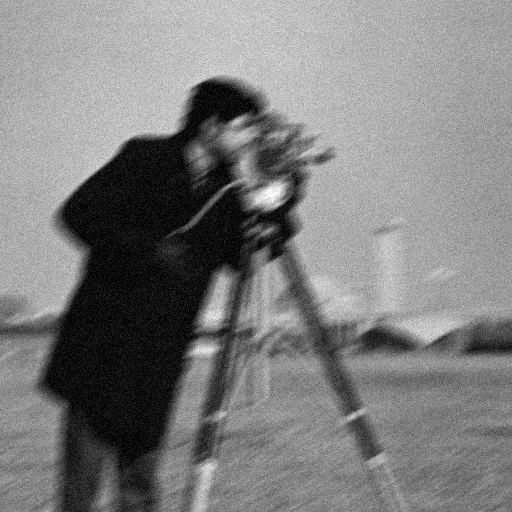
\includegraphics[width=0.32\linewidth]{blurredn.png}}\hfill
    \subcaptionbox{图~\ref{fig:blurredn} 维纳滤波的结果\label{fig:recovered}}{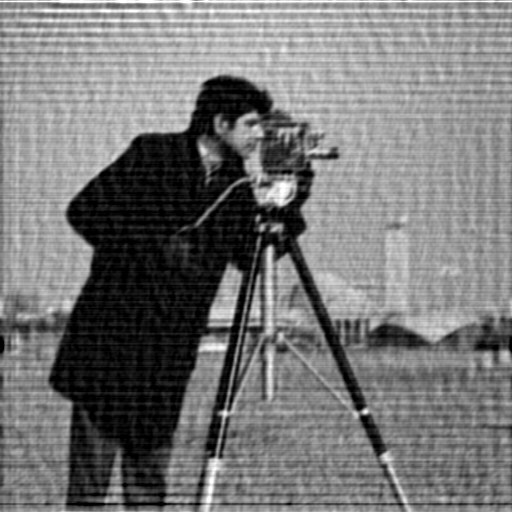
\includegraphics[width=0.32\linewidth]{recovered.png}}\hfill
    \subcaptionbox{对图~\ref{fig:blurredn} 使用$\sigma=0.04$的噪声估计得到维纳滤波的结果\label{fig:recovered4}}{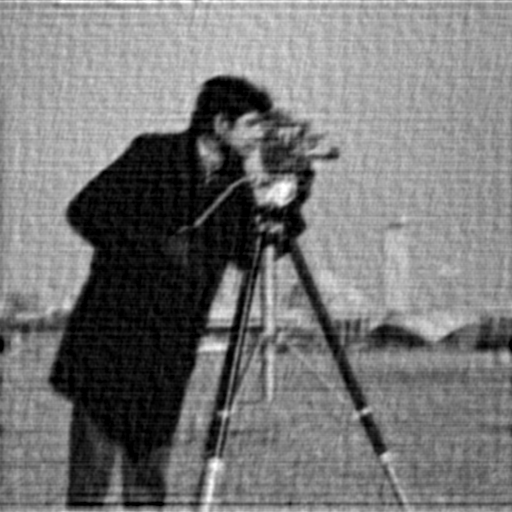
\includegraphics[width=0.32\linewidth]{recovered4.png}}\\
    \subcaptionbox{加入$\sigma=0.1$的白噪声的运动模糊图像\label{fig:blurredn2}}{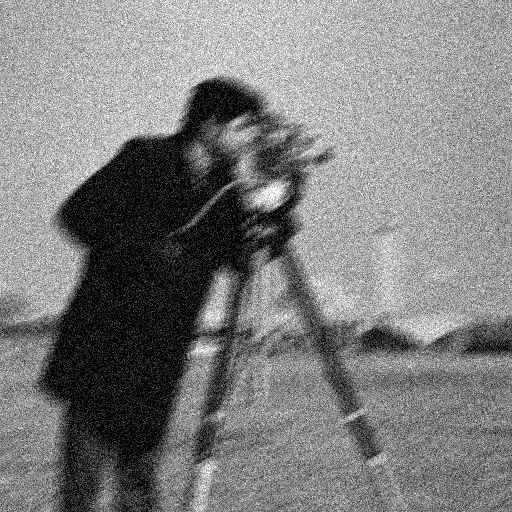
\includegraphics[width=0.32\linewidth]{blurredn2.png}}\hfill
    \subcaptionbox{图~\ref{fig:blurredn2} 维纳滤波的结果\label{fig:recovered2}}{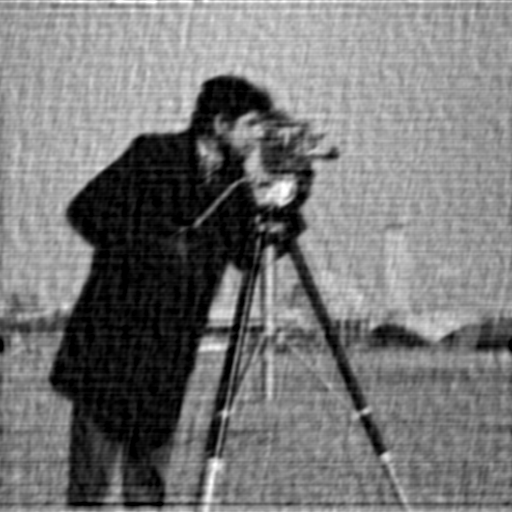
\includegraphics[width=0.32\linewidth]{recovered2.png}}\hfill
    \subcaptionbox{对图~\ref{fig:blurredn2} 使用$\sigma=0.1$的噪声估计得到维纳滤波的结果\label{fig:recovered3}}{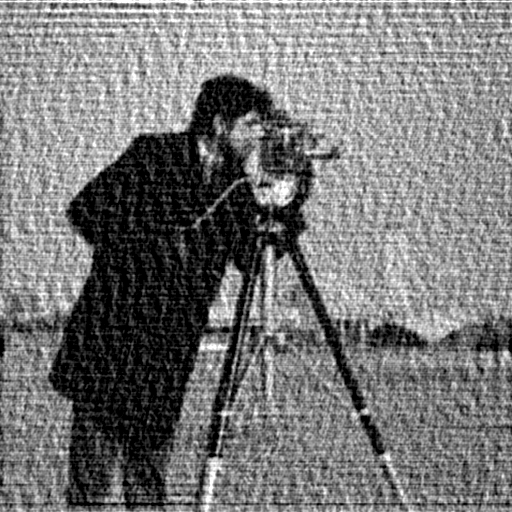
\includegraphics[width=0.32\linewidth]{recovered3.png}}
    \caption{仿真实验结果}
    \label{fig:results}
\end{figure}

仿真实验结果如图~\ref{fig:results} 所示。
图~\ref{fig:origin} 为原图像,图~\ref{fig:blurred} 为未加入噪声的模糊图像。
图~\ref{fig:blurredn} 为加入$\sigma=0.04$的白噪声的运动模糊图像,
对该图像进行直接逆滤波的结果为图~\ref{fig:inverse},其原有的形态已经完全被噪声掩盖,无法分辨;
而对图~\ref{fig:blurredn} 进行维纳滤波的结果为图~\ref{fig:recovered},
虽然边缘存在一定的振铃效应,但原图像中的成分基本清晰可辨,背景中靠中间的建筑物的柱子也完全能分辨清楚;
图~\ref{fig:blurredn2} 为加入$\sigma=0.1$的白噪声的运动模糊图像,
相比图~\ref{fig:blurredn} ,其在视觉上呈现了明显的噪点,内容更难辨认。
对其进行维纳滤波的结果为图~\ref{fig:recovered2},
其后方建筑物的支柱已较难分辨,但从与原图间的均方误差的角度看,并没有同图~\ref{fig:recovered} 之间存在明显的差距。

图~\ref{fig:recovered3} 给出了一种噪声估计与实际噪声不匹配的情况,
这时维纳滤波的效果出现了明显的下降,图像的内容变得难以分辨。
相比之下,图~\ref{fig:recovered4} 虽然也出现了噪声估计与实际噪声的不匹配,
但由于这种估计在噪声模型上和实际保持一致的同时,也提供了一个更紧的约束,因此恢复结果依然很好。

\section{结论}

维纳滤波能在存在噪声的情况下对运动模糊图像进行有效的复原,相比直接逆滤波的的方法存在极大优势,但需要较为准确的噪声以及估计。
同时,在实际运用中,运动模糊的参数也不一定能先验地知道,需要进行估计。
一种行之有效地方案是利用频谱的能量集中特征,利用拉东变换或者霍夫变换对运动模糊的参数进行估计\cite{_radon_2011}。

\printbibliography[heading=bibliography,title=参考文献]

\end{document}
